\section{论文工作是否按开题报告预定的内容及进度安排进行}

\vspace{3mm}
\subsection{论文工作开题预定的研究内容}

\vspace{2mm}
\subsubsection{论文研究背景}
QUIC是一个通用的基于UDP协议的传输层网络协议,最初由Google设计实现并大规模部署\cite{langley2017quic},该协议旨在解决TCP协议的许多问题,减少客户端服务器连接的延迟。
2021年,其于RFC9000\cite{rfc9000}中正式推出标准化版本。
QUIC与HTTP/2的多路复用连接协同工作,允许多个数据流独立到达所有端点,因此不受涉及其他数据流的丢包影响。
QUIC的次要目标包括降低连接和传输时延,以及每个方向的带宽估计以避免拥塞。
HTTP/3是即将到来的第三个主要版本的HTTP协议,将基于QUIC协议实现,现在处于草案阶段。
另外,DoQ(DNS over QUIC)也处于研究阶段。
因此,在QUIC协议的基础上,本课题计划实现一种对抗中间人流量分析攻击的安全链路。

\begin{figure}[h]
  \centering
  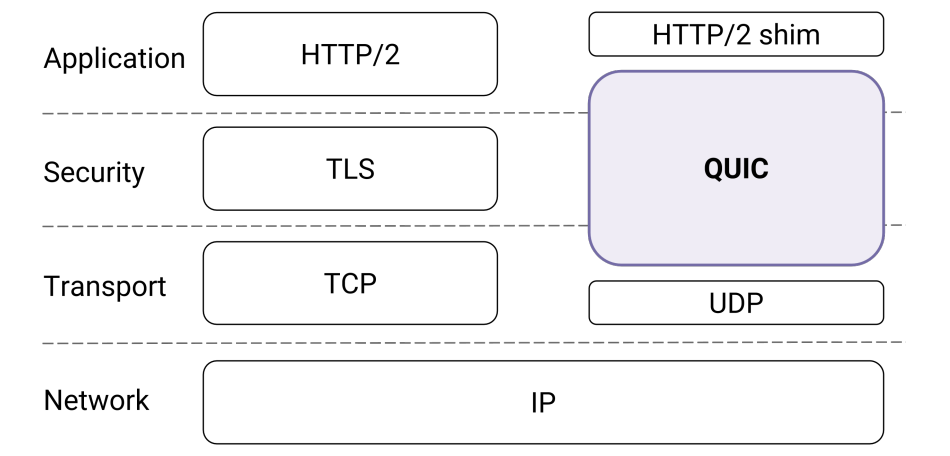
\includegraphics[width=\textwidth]{1}
  \caption{传统HTTPS堆栈与QUIC的对比}
  \label{fig:1}
\end{figure}

\vspace{2mm}
\subsubsection{论文预定研究内容}
本论文计划实现一种基于QUIC的对抗中间人流量分析攻击的安全链路,可以保证客户端与服务器通信的安全性。


\vspace{3mm}
\subsection{现阶段实际的论文工作及进度安排}
目前论文工作按照开题的内容及进度安排推进。
实现了预定的功能的程序代码,实现了预定的功能,与论文工作的进度安排与内容大体一致。 

\begin{table}[h]
  \begin{tabular}{|l|l|}
  \hline
  2022年1月-2022年2月 & \begin{tabular}[c]{@{}l@{}}研究学习QUIC的原理、特点,了解其相比TLS/TCP的优势\end{tabular}  \\ \hline
  2022年3月-2022年4月   & \begin{tabular}[c]{@{}l@{}}代码实现一种对抗中间人流量分析攻击的安全链路\end{tabular}       \\ \hline
  2022年5月         & \begin{tabular}[c]{@{}l@{}}根据测试的结果,进一步优化程序 \end{tabular} \\ \hline
  2022年6月         & 整理论文,完成结题报告。                                      \\ \hline
  \end{tabular}
\end{table}

\vspace{8mm}
\section{已完成的研究工作及结果}
目前已经实现了预定功能的全部代码,基本完成了预定的目标,下面是主要完成的成果:

\vspace{3mm}
\subsection{可靠加密隧道}
由于QUIC基于TLS1.3,因此客户端和服务器在传输数据前先要经过密钥协商握手,之后双方通信的数据都经过共同协商的密钥加密传输。
TLS握手后,通信双方建立起一条安全的加密隧道。TLS 1.3采用的AEAD加密算法,保证了认证加密(Authenticated encryption),这是一种能够同时保证数据的保密性、完整性和真实性的一种加密模式。
本课题选用了其中的TLS\_CHACHA20\_POLY1305\_SHA256作为通信双方使用的加密算法。

\vspace{3mm}
\subsection{对抗流量分析攻击}
QUIC有多路复用连接(Multiplexing)的特性,允许多个数据流独立到达所有端点,因此不受涉及其他数据流的丢包影响。
客户端与服务器建立起一个连接(session),通过该连接传输的数据以一个个stream的形式传输,不同stream完全自主,一个stream数据包的丢失不影响其他stream数据包的发送。
客户端在与服务器握手结束后,用户程序与客户端的一个TCP连接,等同于客户端与服务器的一个连接的stream。
因此,在隧道传输的UDP数据包难以识别其包含的数据报文信息,保证了对抗流量分析攻击的安全性。

\vspace{3mm}
\subsection{密码认证}
目前服务器并发支持多个客户端连接,服务器与单个客户端需要预先设置共享的密码。
客户端与服务器第一次TLS握手结束后,服务器通过验证客户端发送的密码(加密传输),选择终止该连接或者建立连接成功,之后建立的0-RTT连接不需要密码认证这一步。
如下图所示,客户端与服务器第一次握手是1-RTT,建立连接后的握手都是0-RTT,意味着数据不需要等到握手结束后才能发送,可以直接加密发送。

\begin{figure}[h]
  \centering
  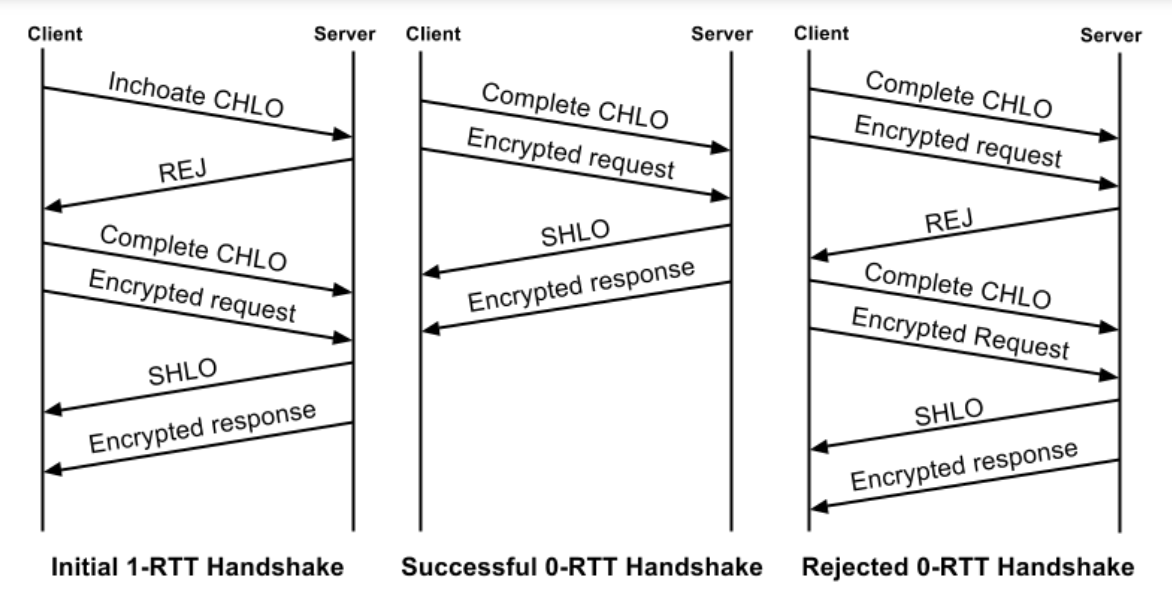
\includegraphics[width=\textwidth]{2}
  \caption{QUIC的初始1-RTT握手、随后成功的0-RTT握手和失败的0-RTT握手}
  \label{fig:1}
\end{figure}

\vspace{3mm}
\subsection{API控制}
目前初步设计完成了程序的RESTful API,程序在运行的同时会在一个端口运行API服务器。
在不重启程序的前提下,可以通过访问API接口获取程序运行的一些信息,同时也能控制程序内部的配置。
基于API,程序运行时会在同一个端口运行静态网页服务器,用户可以通过浏览器打开相应页面,通过GUI完成API接口的功能。

\vspace{3mm}
\subsection{多种模式选择}
目前支持直连(Direct)、规则(Rule)、代理(Global)三种模式,直连类似透明代理,
代理模式选择代理所有的请求。规则模式基于简单的isocode匹配,通过geolite2数据库得到IP地址对应的国家isocode,
根据作出直连或者代理的选择。

\vspace{3mm}
\subsection{低延迟}
相较于TLS/TCP,建立在QUIC的安全连接有低延迟的优点。
使用TLS/TCP,通信双方建立一条安全连接,需要经过TCP3次握手和
TLS 1.2握手共消耗3次往返时间(RTT)。尽管有TCP Fast Open\cite{radhakrishnan2011tcp}和TLS1.3可以改进,但需要额外的配置,在实际部署也有许多问题。
而使用QUIC初次建立安全连接,需要1-RTT,之后甚至只需要0-RTT,意味着数据可以不需要等待TLS1.3握手结束直接发送。


\vspace{3mm}
\subsection{容器化}
目前对实现的客户端和服务器程序通过Docker都实现了对应用程序的打包,
保证了在其他主机通过Docker可以运行程序。

\vspace{8mm}
\section{后期拟完成的研究工作及进度安排}

\vspace{3mm}
\subsection{后期待完成工作}
\begin{enumerate}
  \item 目前初步在API接口实现了查看、修改设置的功能,计划进一步完善功能。
  \item 现在实现的0-RTT还有些问题,第一次连接后的新连接有一部分不是0-RTT,准备解决这个问题。
  \item 目前测试还比较少,目标增加测试用例,提高对程序测试的覆盖率。
  \item 完成毕业论文,进行终期答辩。
\end{enumerate}

\vspace{3mm}
\subsection{进度安排}

\begin{table}[h]
  \begin{tabular}{|l|l|}
  \hline
  2022年3月-2022年4月   & \begin{tabular}[c]{@{}l@{}}代码实现一种对抗中间人流量分析攻击的安全链路\end{tabular}       \\ \hline
  2022年5月         & \begin{tabular}[c]{@{}l@{}}增加对程序的测试,根据测试的结果,进一步优化程序 \end{tabular} \\ \hline
  2022年6月   & 整理论文,完成结题报告。                                      \\ \hline
  \end{tabular}
\end{table}

\vspace{8mm}
\section{存在的问题与困难}

\vspace{3mm}
\subsection{程序优化}
相较于TLS/TCP,QUIC由于1-RTT甚至0-RTT的特性,在短连接与传输数据少于1MB的连接有一定优势,在长连接与传输大于1MB数据的优势不明显。

由于TCP在内核层面的优化,UDP在内核优化的方面还有许多改善的空间。另外,相较于UDP,TCP有许多硬件层面的优化(零复制),这也造成基于UDP的QUIC在硬件层面的性能差距。
QUIC在应用程序空间中实现,而不是在操作系统内核中实现。虽然这可以使得算法得到更快的改进,但同时会带来更多的用户空间与内核空间的上下文切换,增加了额外的开销。

目前正在学习和进行对其的优化。程序优化

\vspace{3mm}
\subsection{API接口和GUI}
目前的API接口可以查看、修改程序运行的配置,目前在考虑加入更多功能,比如查看程序运行日志,连接情况等。

同时,目前实现的网页控制端还比较简单,最近正在学习相关的一些知识,准备进一步完善GUI。


\vspace{3mm}
\subsection{0-RTT实现}
理论上,第一次连接认证后,之后的连接都是0-RTT。
但现在代码实际运行还有些问题,在某一时间如果并发开启多个连接,只有一半的连接是0-RTT,其他的是1-RTT。
因此,在目前测试情况下,大概2/3的连接是0-RTT。

\vspace{8mm}
\section{论文按时完成的可能性}
目前已经按照计划对主要功能的代码进行实现,还需要一些优化和GUI美化,
按照进度安排解决现阶段出现的问题并逐步推进未完成的工作,论文可以按时完成。 

\vspace{8mm}
\section{主要参考文献}

\bibliographystyle{hithesis}
\bibliography{references}
